% options:
% thesis=B bachelor's thesis
% thesis=M master's thesis
% czech thesis in Czech language
% slovak thesis in Slovak language
% english thesis in English language
% hidelinks remove colour boxes around hyperlinks


\documentclass[thesis=B,czech]{FITthesis}[2012/06/26]

\usepackage[utf8]{inputenc} % LaTeX source encoded as UTF-8

\usepackage{graphicx} %graphics files inclusion
% \usepackage{amsmath} %advanced maths
% \usepackage{amssymb} %additional math symbols

\usepackage{dirtree} %directory tree visualisation



% % list of acronyms
% \usepackage[acronym,nonumberlist,toc,numberedsection=autolabel]{glossaries}
% \iflanguage{czech}{\renewcommand*{\acronymname}{Seznam pou{\v z}it{\' y}ch zkratek}}{}
% \makeglossaries

\newcommand{\tg}{\mathop{\mathrm{tg}}} %cesky tangens
\newcommand{\cotg}{\mathop{\mathrm{cotg}}} %cesky cotangens

% % % % % % % % % % % % % % % % % % % % % % % % % % % % % % 
% ODTUD DAL VSE ZMENTE
% % % % % % % % % % % % % % % % % % % % % % % % % % % % % % 

\department{Katedra softwarového inženýrství}
\title{Systém pro analýzu proudu dat v reálném čase}
\authorGN{David} %(křestní) jméno (jména) autora
\authorFN{Viktora} %příjmení autora
\authorWithDegrees{David Viktora} %jméno autora včetně současných akademických titulů
\supervisor{Ing. Adam Šenk}
\acknowledgements{Poděkování ....}
\abstractCS{V~několika větách shrňte obsah a přínos této práce v~češtině. Po přečtení abstraktu by se čtenář měl mít čtenář dost informací pro rozhodnutí, zda chce Vaši práci číst.}
\abstractEN{Sem doplňte ekvivalent abstraktu Vaší práce v~angličtině.}
\placeForDeclarationOfAuthenticity{V~Praze}
\declarationOfAuthenticityOption{4} %volba Prohlášení (číslo 1-6)
\keywordsCS{Nahraďte seznamem klíčových slov v češtině oddělených čárkou.}
\keywordsEN{Nahraďte seznamem klíčových slov v angličtině oddělených čárkou.}


\begin{document}

% \newacronym{CVUT}{{\v C}VUT}{{\v C}esk{\' e} vysok{\' e} u{\v c}en{\' i} technick{\' e} v Praze}
% \newacronym{FIT}{FIT}{Fakulta informa{\v c}n{\' i}ch technologi{\' i}}

\begin{introduction}
	Kratce o jednotlivých bodech zadání a struktuře prace, motivace
	
\end{introduction}

%\chapter
%\section
%\subsection
%


\chapter{Situace v oblasti zpracovávání dat}
	V současné době generujeme obrovská množství dat - podle některých odhadů to například v roce 2012 mohlo být až 2,5 exabajtů za den\cite{bbc-bigdata}. Od té doby se rychlost přibývání dat stále zvyšuje. Například nárůst objemu dat dostupných na internetu je způsoben jeho neustále větším rozšířením a rostoucí dostupností. V  roce 2016 je k němu připojeno již přes 3,3 miliardy obyvatel planety\cite{internet-live-stats}, což je téměř polovina všech. Roste také míra využívání internetu. Oproti dřívějšku na internetu trávíme nejen díky chytrým telefonům stále více času a využíváme například sociální sítě, internetové vyhledávání a další online služby. Během toho jsou nám zobrazována personalizovaná data a cílené reklamní nabídky. Také ve firemní i státní sféře výrazně roste stupeň využívání informačních technologií a v návaznosti na to objem produkovaných dat. S přibývajícími daty nastávají problémy s jejich zpracováním. Jedním z nich je obecně schopnost zpracovat tak veliké objemy dat, druhým je schopnost jejich zpracování v dostatečně krátkém, ideálně reálném čase. Často je přitom potřeba vyřešit oba tyto problémy naráz. Pro popis těchto dat a problémů spojených s jejich zpracováním se používá relativně nový pojem Big Data. 

		 
\section{Big Data a technologie pro práci s nimi}
	Právě pojem Big Data je často označován za jeden z největších buzzwords\footnote{Slova nebo fráze, které jsou v současné době populární} současného IT světa. I přes jeho popularitu nejsou přesně vymezené jeho hranice či definované pojmy zabývající se toutu oblastí. Obecně můžeme říci, že o Big Datech hovoříme v případech, kdy je potřeba zpracovávat objemy dat v řádech gigabajtů a více. To je velice zjednodušený popis tohoto termínu, přesná definice však neexistuje a na celý problém se dá dívat různými způsoby. Rozšířené je například také tvrzení říkající, že o Big Datech mluvíme zkrátka v těch případech, kdy klasické databázové a softwarové nástroje především kvůli objemu těchto dat selhávají\cite{webopedia-bigdata}. 

	Přestože jednotná definice neexistuje, ustálilo se několik problémů, kterým je při práci s Big Daty potřeba čelit. Jedná se o takzvaná 3+1V - Volume, Velocity, Variety a později přidaná vlastnost Veracity\cite{dp-customer-inteligence}. Volume popisuje objem zpracovávaných dat, Velocity pak rychlost, jakou data přibývají. Charakteristikou Variety popisujeme různorodost dat a Veracity určuje úplnost a míru důvěryhodnosti dat. Ne vždy se setkáme se všemi těmito problémy naráz, každá z nich ale přidává na složitosti zpracování těchto dat. 
	
	Právě kvůli těmto vlastnostem se při práci s velkými objemy dat klasické technologie používané v minulosti stále častěji ukazují jako nedostatečně rychlé nebo obecně neschopné tato data zpracovat. Je proto nutné sáhnout po nových technologiích určených pro práci s nimi. Bez technologií pro Big Data se v dnešní době neobejdou třeba již zmiňované internetové vyhledávače nebo sociální sítě, využití ale nacházejí i v mnoha dalších oblastech. Jejich rozvoj je také předpokladem například pro další rozšíření tzv. Internet of Things\cite{bigdata-iot}.  

\subsection{Strukturovaná a nestrukturovaná data}	
	Data obecně často rozdělujeme do dvou kategorií - na data strukturovaná a nestrukturovaná. Strukturovaná data jsou obvykle uložena v klasické relační databázi, nebo obecně utříděna po řádcích a s přesně definovanými sloupci. Ostatní data, která nemají takto pevně danou strukturu, jsou data nestrukturovaná. Ještě donedávna docházelo ke zpracování téměř váhradně dat strukturovaných. Ta nestrukturovaná však často nabízejí obrovský potenciál k jejich využití. Klasickým příkladem nestrukturovaných dat je lidská řeč v psané formě - ta rozhodně obsahuje spoustu informací, ale ve formě kterou je počítačově složité analyzovat. Může se jednat například o články, konverzace nebo příspěvky na sociálních sítích.  Právě příspěvkům na sociální síti Twitter se věnuje i tato práce. 
	
	Analýzou lidské řeči se zabývá obor zvaný Natural Language Processing, obecně vytěžováním znalostí z dat pak tzv. Data Mining. Často skloňovaným pojmem je také Machine Learning, v češtině strojové učení. Pro všechny tyto obory jsou technologie pro Big Data obrovským přínosem - díky nim je možné získat opravdu cenné informace snáze a rychleji než bylo možné dříve. Například analýzou dat pohybu uživatele po webové stránce a jeho chováním můžeme odhalit nedostatky tohoto webu a jejich odstraněním zvýšit míru konverze. Hovoříme-li v kontextu sociální sítě Twitter, možnosti jsou ještě zajímavější. Na základě příspěvků a vyplněných informací jednotlivých uživatelů můžeme například odhadovat jejich volební preference nebo nabízet velice přesně cílenou reklamu. Konkrétnějším příkladem může být zajímavý projekt ze Stanfordské univerzity usilující o odhad vývoje cen akcií na základě analýzy sentimentu příspěvků z Twitteru\cite{stock-stanford}. Touto technikou se budu zabývat v následující kapitole této práce.  

	Technologie pro Big Data je samozřejmě možné použít i na data strukturovaná, největší využití však nabízejí při zpracování těch nestrukturovaných. Protože nestruktorovaná data přibývají výrazně rychleji\cite{structured-unstructured}, a protože je jejich zpracování obvykle výpočetně náročnější, jsou právě technologie pro Big Data vhodnou volbou. 
 
	
\subsection{Principy zpracování velkých dat}
	Jedny z prvních konkrétních technologií pro práci s Big Daty vznikaly na přelomu tisíciletí ve společnosti Google. Právě Google v roce 2004 zveřejnil článek o modelu MapReduce\cite{mapreduce-google}, která se stala stavebním kamenem pro většinu dalších technologií pro práci s velkými objemy dat. MapReduce vlastně popisuje dvě nezávislé funkce. První z nich je funkce Map, ve které jsou ze vstupních dat vygenerovány dvojice klíč a hodnota. Poté co je funkce Map dokončena, její výstup je použit jako vstup do funkce Reduce. Ta pak spojí vstupní data podle klíče\cite{mapreduce-description}. 
	
	Klíčovou vlastností MapReduce modelu je možnost paralelizace Map fáze na počítačovém clusteru. Jeden z počítačů v clusteru například přijme požadavek od uživatele. Tento počítač rozdělí vstupní data ostatním počítačům v clusteru a vyčká na provedení Map fáze těmito počítači. Výsledná data pak sám master spojí v Reduce fázi a navrátí výsledek uživateli. Distribuce co největšího množství operací a výpočtů po počítačovém clusteru je v dnešní době obecně hlavním principem fungování technologií pro zpracování velkých objemů dat. Paradoxně nemusí jít o dražší řešení než nákup jednoho supervýkoného serveru. Clustery pro práci s Big Daty jsou totiž obvykle tvořeny běžně dostupnými a relativně levnými servery. 
	
	\begin{figure}[ht]
    	\centering
    	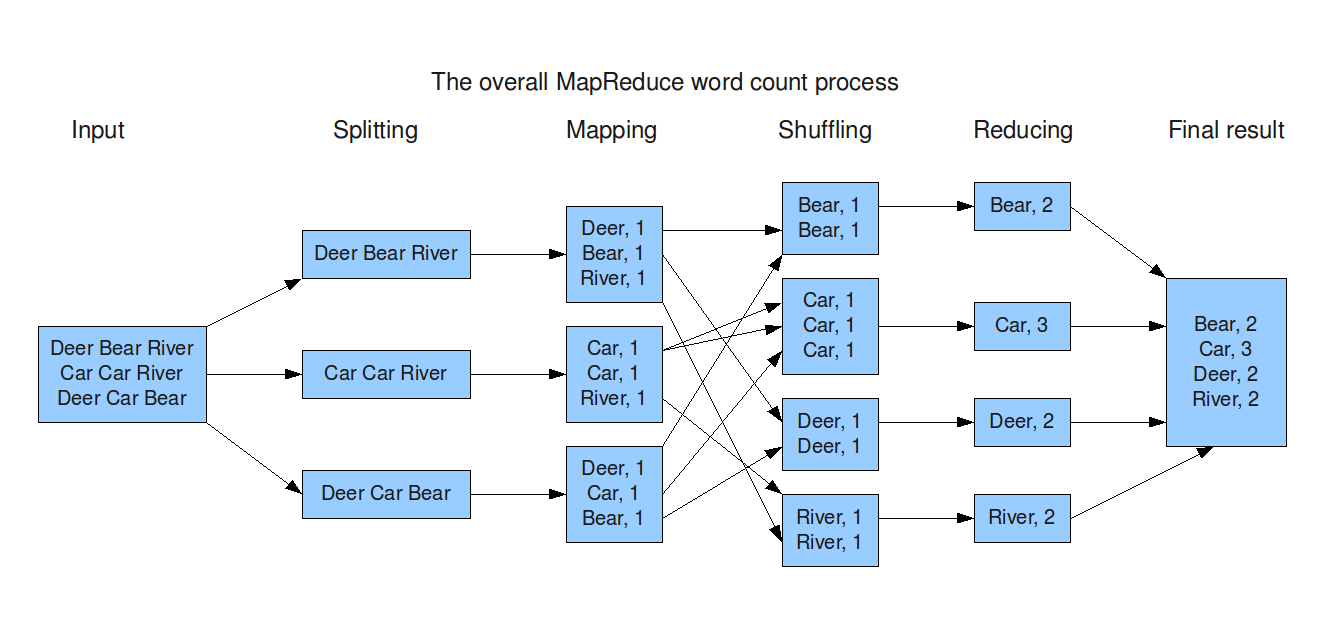
\includegraphics[width=1\textwidth]{images/mapreduce.png}
    	\caption{Ukázka fungování MapReduce paradigmatu \cite{mapreduce-img} }
    	\label{fig:mapreduce}
	\end{figure}
	
	Především v posledních letech se objevují konkrétní komplexnější nástroje pro práci s velkými daty. Tyto nástroje obvykle obsahují i další technologie, mimo jiné umožňující například správu a konzistenci počítačového clusteru. Tyto frameworky principielně data zpracovávají dvěma různými způsoby - jde o tzv. batchové zpracování nebo o zpracování streamové. 
	
\subsection{Batchové zpracování Big dat}
	Batchové nebo-li dávkové zpracování je vhodné především pro takové úkoly, jejichž výsledky není nutné znát ihned. Data jsou nejprve po určitou dobu shromažďována a až poté je jednorázově spuštěna úloha pro jejich zpracování. Toto zpracování obvykle zabere relativně dlouhý čas. Zmiňovaný MapReduce se využívá právě pro batchové zpracování dat. 

	Jedním z prvních klíčových frameworků který umožnil další vývoj v oblasti Big dat je jednoznačně open-source framework Hadoop\cite{hadoop-home}. Protože využívá MapReduce model podporuje právě batchové zpracování dat. Jeho první plná verze vyšla na konci roku 2011, ale byl využíván již přibližně od roku 2006 například ve společnosti Yahoo\cite{hadoop-history}. Je určen pro použití na počítačových clusterech složených z řádově desítek až stovek běžně dostupných serverů. Hadoop se skládá ze tří hlavních komponent - Hadoop Distributed File System, Hadoop MapReduce a Hadoop YARN. HDFS neboli Hadoop Distributed File System je distribuovaný filesystem zajišťující rozprostření dat po jednotlivých počítačích v clusteru. Klade důraz na toleranci výpadků částí clusteru. Pro zabránění ztráty dat v případě takového výpadku dochází mimo jiné k jejich replikaci na více strojů. Hadoop MapReduce je konkrétní implementace MapReduce modelu zmiňovaného dříve. Hadoop YARN pak slouží především k řízení zdrojů v clusteru, tedy například rozdělování práce jednotlivým serverům v clusteru. Nevýhodou Hadoopu je fakt, že nepodporuje proudové zpracování dat, ale pouze zpracování batchové. 
	
	V současné době jsou k dispozici i další batchově zaměřené frameworky, které často dosahují lepších výsledků než Hadoop a mimojiné obvykle umožňují vytváření úloh na vyšší úrovni. Díky ním například není nutné přímo vytvářet mapovací a reduce funkci. Nejrozšířenějím je bezesporu Apache Spark\cite{spark-home}, kterému se budu podrobněji věnovat v následujících sekcích. Oproti Hadoopu dosahuje především díky cachování a dalším vylepšením často několikanásobně kratší doby zpracování. Krom batchového zpracování umožňuje i práci s proudy dat. 

\subsection{Streamové zpracování}
	V praxi často potřebujeme velké objemy dat zpracovávat v co nejkratším čase a ideálně na každý nový podnět co nejdříve zareagovat. Batchové zpracování je v takovém případě nevhodné. Řešením je již zmiňované streamové zpracování, nebo také zpracování proudů dat. Vstupem do takového programu není fixní soubor dat, ale neustálý proud dat nových. Kdykoli program obdrží nový datový objekt, zjednodušeně ho začne okamžitě zpracovávat a mezivýsledky předávat mezi jednotlivými částmi programu nezávisle na dalších vstupech. Technologií umožňujících streamové zpracování velkých objemů dat je několik, ty nejzajímavější jsou ale Apache Spark, Apache Storm a Apache Flink. Každá z těchto technologií funguje na trochu jiném principu a je vhodná pro jiné využití. 
	
	Apache Flink je nejnovějším frameworkem, který v relativně velké míře konkuruje Sparku. Stejně jako Spark, podporuje Flink oba způsoby zpracování dat, primárně je ale zaměřený na streamy. Narozdíl od Sparku ale podporuje streamové zpracování v pravém slova smyslu a lze s ním tak dosáhnout výrazně kratší doby zpracování\cite{streaming-benchmark}. I právě proto se předpokládá, že v oblasti zpracování proudů dat v budoucnu předstihne Spark\cite{flink-future}. Jeho další výhodou je například možnost využití existujících programů pro Storm či MapReduce. Hlavní nevýhodou je momentálně fakt, že je teprve v počátcích svého vývoje a často se tak uživatel může setkat s bugy či chybějící dokumentací. 
	
	Apache Storm jako jediný ze zmiňovaných frameworků nabízí pouze streamové zpracování, i on však poskytuje pravé streamové zpracování. Jeho API je oproti Flinku více nízkoúrovňové a vývoj v něm tak může být pracnější. Obecně ale funguje na podobném principu jako právě Flink. Oproti zbývajícím dvěma technologiím Storm postrádá například tzv. Streaming Windows a další funkce\cite{so-flink-storm}.
	
	Rozhodně nejrozšířenější technologií s největší komunitou a pokočilejším stupněm vývoje je Apache Spark. Tomu se podrobněji věnuji v další sekci. Pro porovnání s dalšími technologiemi ale lze říct, že v oblasti proudového zpracování se hodí především pro ty případy užití, kdy není nutné co nejrychlejší zpracování a řádově několikasekundové zpoždění nehraje roli. Je pak momentálně oproti zbylým technologiím vhodnou volbou díky svojí vyspělosti a jednoduchosti. Pokud je ale nutné opravdu real-time zpracování, je třeba volit mezi Flinkem a Stormem. Ty fungují na podobném principu, nicméně Flink má některé funkcionality, které ve Stormu chybí\cite{so-flink-storm}. Flink také nabízí vysokoúrovňové API a do budoucna se jeví jako perspektivnější framework. 
	
	
	
\section{Apache Spark}
	Apache Spark je open-source framework pro distribuované zpracování dat. Vznikl na Kalifornské univerzitě v Berkeley, která ho v roce 2013 věnovala Apache Software Foundation. V rámci této nadace je Spark momentálně jedním z nejaktivněji vyvýjených projektů\cite{spark-toplevel}. Poskytuje API pro jazyky Java, Scala, Python a nově také R. Jak již bylo řečeno, Apache Spark podporuje batchové i proudové zpracování dat. 
	
	Primárně je Spark zaměřený na batchové zpracování, ve kterém může Hadoop až několikanásobně překonat svou rychlostí. Toho dosahuje několika vylepšeními - především nepoužívá přímo MapReduce paradigma, které je v některých ohledech příliš svazující, ale vlastní algoritmy založené na podobných principech ale navržené odlišným způsobem. Hadoop například výsledky většiny operací ukládá na disk, kdežto Spark často využívá cachování a operační pamět. Je pak na operačním systému, jestli se rozhodne tato data zapsat na disk\cite{spark-mapreduce-difference}. Právě využívání operační paměti pak samozřejmě vede k výraznému zrychlení. 
		
	Spark narozdíl od Apache Flink a Apache Storm nenabízí plnohodnotné proudové zpracování, ale takzvané micro-batchové zpracování. Spark nereaguje na každý nový datový objekt samostatně, ale nejdříve data po zadanou dobu střádá a poté je víceméně klasicky batchově zpracuje. Tento proces je pak neustále opakován. Oproti klasickému batchovému zpracování je interval sběru dat obvykle várazně kratší.  Přestože Spark při zpracování proudů dat obvykle nedosahuje takových rychlostí jako právě Flink nebo Storm, i s ním je možné dosáhnout zpracování dat v téměř reálném čase\cite{streaming-benchmark}. 

	Stejně jako Hadoop využívá i Spark další technologie pro správu clusteru a distribuované ukládání dat. Jeho velikou výhodou je možnost výběrů mezi několika. Pro správu clusteru je možné využít cluster manager integrovaný přímo do Sparku, Hadoop YARN nebo Apache Mesos. Pro distribuované ukládání je pak výběr ještě rozsáhlejší, volit lze mezi již zmiňovaným HDFS, Cassandrou, OpenStack Swift, Amazon S3, Kudu nebo MapR-FS. Především při vývoji se pak hodí možnost využití pseudo-distribuovaného režimu, při kterém není žádný z těchto systémů potřeba. Spark totiž při tomto nastavení běží na jediném počítači v režimu, kdy jedno jádro odpovídá jednomu klientskému počítači v clusteru. 

\subsection{Komponenty frameworku}
	Jak znázorňuje obrázek \ref{fig:spark_components}, Apache Spark se skládá z několika hlavních komponent. 
		\begin{figure}[ht]
    	\centering
    	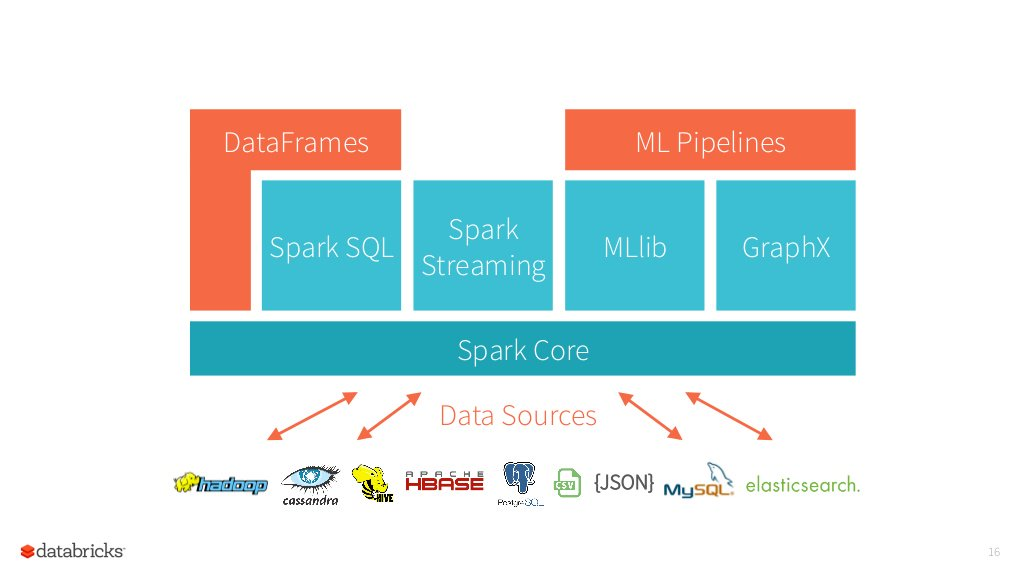
\includegraphics[width=1\textwidth]{images/spark_engine.jpg}
    	\caption{Komponenty frameworku Spark\cite{spark-components}}
    	\label{fig:spark_components}
	\end{figure}
	
\subsubsection{Spark core}
	Tou hlavní komponentou je Spark Core, který zajišťuje všechny základní funkcionality Sparku, jako jsou například plánování úloh a základní vstupní a výstupní operace. Ostatní komponenty nad ním staví. Základním pojmem je zde tzv. Resilient Distributed Dataset, nebo-li RDD. RDD je zjednodušeně řeřeno téměř libovolná kolekce dat, nad kterou je možné provádět paralelní výpočty. Je navíc zajištěna jejich konzistence - při výpadku některého ze strojů mohou být ztracená data obnova pomocí informací na těch ostatních. 
	
	Kdykoli je na konkrétním RDD vykonána některá z operací umožňujících paralelní zpracování, tzv. transformace (například map, filter nebo reduce), driver nebo-li počítač řídící ostatní počítače naplánuje její zpracování na všech počítačích v clusteru. Ty poté vytvoří nová RDD s výsledky. Operace na RDD jsou ale "lazy", což znemaná, že se neprovádějí dokud na RDD neaplikujeme nějakou akci. Akce je opakem transformace a jejím výsledkem není vytvoření nového RDD. Příkladem akce je vypsání obsahu RDD na standartní výstup. 

\subsubsection{Spark SQL}
	Další důležitou komponentou je Spark SQL, dříve nazývaný jako Apache Shark. Ten umožňuje práci s především strukturovanými daty. Zavádí také novou strukturu zvanou Data Frame (DF). Stejně jako RDD, je i Data Frame distribuovaný po clusteru. Jeho struktura je ale narozdíl od RDD pevně daná - konceptuelně odpovídá klasické tabulce v relační databázi. Vnitřně v něm dochází k optimalizacím urychlujícím operaci s ním. 
	
	Hlavní předností Spark SQL je možnost používat klasické SQL nebo HiveQL\footnote{An example footnote.} dotazy, jejichž výsledky jsou uloženy právě jako Data Frame. Například komunikace s klasickou relační databází je možná pomocí JDBC/ODBC\footnote{An example footnote.}. 


\subsubsection{Spark Streaming}
	Jak již bylo řečeno, Spark neumožňuje streamové zpracování v pravém slova smyslu, ale pracuje na principu tzv. micro-batchového zpracování. To způsobuje mírné zpoždění výsledků, ty ale nepotřebujeme znát vždy opravdu ihned. Velikou výhodou je fakt, že programy určené pro streamové zpracování se ve Sparku téměř neliší od těch určených k jednorázovému spuštění. 

	\begin{figure}[ht]
    	\centering
    	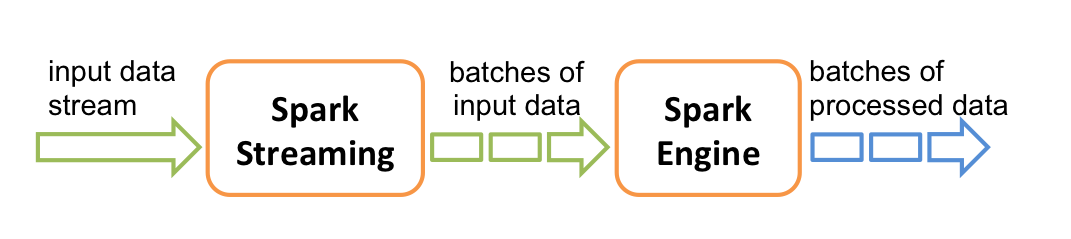
\includegraphics[width=1\textwidth]{images/spark-streaming-flow.png}
    	\caption{Princip fungování Spark Streaming\cite{streaming-guide}}
    	\label{fig:spark_streaming_flow}
	\end{figure}
	
	Jak ukazuje obrázek \ref{fig:spark_streaming_arch}, jako zdroj dat pro Spark Streaming může posloužit například Kafka, Flume, HDFS, Amazon S3 nebo Kinesis. Přímo lze také využívat data z Twitteru bez nutnosti používání dalších knihoven. Právě Twitter poslouží jako zdroj dat pro systém na který se zaměřuje tato práce.  

	\begin{figure}[ht]
    	\centering
    	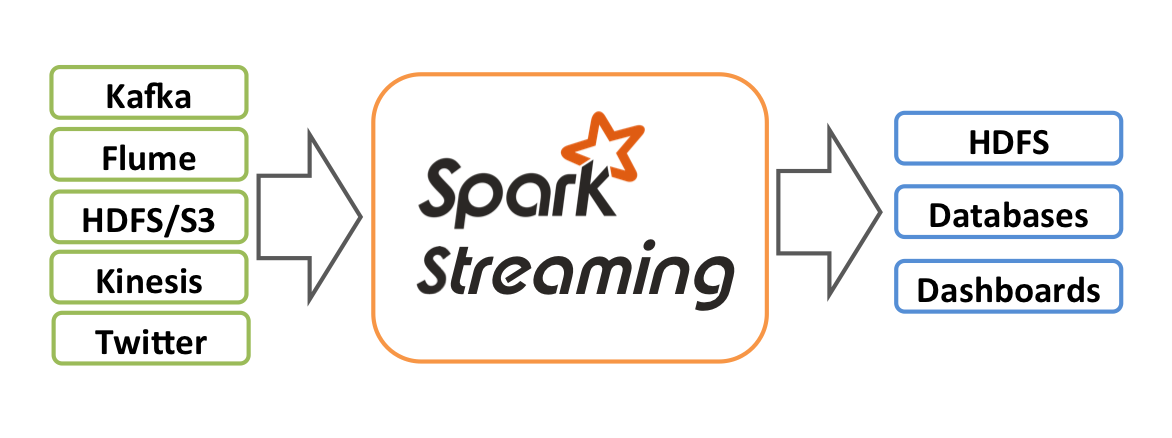
\includegraphics[width=1\textwidth]{images/spark-streaming-arch.png}
    	\caption{Možné zdroje dat a úložiště výsledků pro Spark Streaming\cite{streaming-guide}}
    	\label{fig:spark_streaming_arch}
	\end{figure}
	
	I Spark Streaming zavádí novou strukturu. Nazývá se Discretized Stream nebo-li DStream. Jde o nekonečnou posloupnost nových dat reprezentovaných jednotlivými RDD. Při psaní konkrétních programů pak stačí nastavit délku intervalu, ve kterém se má opakovaně spouštět daná úloha. DStream pak v každém intervalu dané délky vrátí právě jedno RDD, které je již možné klasicky zpracovat. 
	

\subsubsection{MLlib}
	MLlib je framework určený pro strojové učení. Právě díky vlastnostem Sparku (především díky využívání operační paměti) poskytuje výrazně lepší výsledky než klasické technologie pro machine learning. Výhodou tohoto frameworku je to, že v něm jsou již naimplementovány nejpoužívanější algoritmy. Není tak nutná jejich reimplementace uživatelem. 

	
\subsubsection{Graphx}
	GraphX je ve Sparku relativně novým modulem, který je určený obecně pro práci s grafy a paralelními grafovými výpočty. Grafové výpočty získávají stále více pozornosti, jednoduchým příkladem je algoritmus PageRank, který stál u zrodu moderního vyhledávání v Google\cite{google-pagerank}. 
	


%\section{Způsoby zpracování velkých objemů dat}
%	Batchové/streamové, proc se v mem pripade hodi streamove




\chapter{Analýza}
\section{Metody pro analýzu textu}
	Sentiment, ...

\section{Požadavky na systém}
	Výsledný systém, jehož vytvoření je cílem této práce, se bude skládat ze tří klíčových částí - systému pro analýzu textu, databáze a webserveru zpřístupňujícího data pomocí RESTového API.
	
	 První zmiňovaná část, systém pro analýzu textu, bude využívat framework Apache Spark. Jako zdroj dat bude použita sociální síť Twitter poskytující vzorek přispěvků z ní, tzv. tweetů, pomocí veřejného API. Tomu se podrobněji věnuji v kapitole \ref{twitter-api}. Z těchto příspěvků budou vyfiltrovány ty, které reprezentují přání jejich autorů. Kromě měření běžných statistik bude systém provádět analýzu sentimentu těchto přání. Tato analýza bude probíhat v reálném čase, respektive se zpožděním v řádu maximálně několika desítek sekund.  Výsledky analýzy z této části budou persistovány ve vhodné relační databázi. Na ní bude napojen webový server zpřístupňující data pomocí RESTful API. 

\subsection{Funkční požadavky}
\subsubsection{Systém pro analýzu textu}
Samotný systém pro analýzu textu musí splňovat následující požadavky:
\begin{itemize}
\item Získání a ukládání veškerých dat, jejichž zpřístupnění pomocí RESTového API je požadováno a jež nejsou získávána jiným způsobem
\end{itemize}
\subsubsection{Databáze}
 Databáze bude poskytovat následující funkcionality:
\begin{itemize}
\item Agregace statistických dat dle času - u dat u kterých je to možné bude docházet k jejich seskupovaní po větších intervalech. Tím dojde ke snížení náročnosti dotazů na tato data. 
\item Promazávání starých a již zagregovaných dat
\end{itemize}
\subsubsection{RESTful API}
RESTful API bude poskytovat následující data:

\begin{itemize}
\item Jednotlivá přání a základní informace o nich, včetně jejich sentimentu a informací o jejich autorovi
\item Seznam uživatelů zmíněných v konkrétním přání
\item Seznam hastagů použitých v konkrétním přání
\item Informace o uživatelích, kteří jsou autory některého přání nebo byli v některém zmíněni
\item Seznam přání publikovaných daným uživatelem
\item Seznam přání v nichž byl daný uživatel zmíněn
\item Seznam přání obsahujících daný hashtag
\item Statistiky nejpouívanějších hashtagů
\item Statistiky nejvíce zmiňovaných uživatelů
\item Statistiky o počtech již analyzovaných tweetů, anglických tweetů a z nich vyfiltrovaných přání v daném časovém intervalu
\item Statistika o průměrném sentimentu v daném intervalu
\end{itemize}

\noindent Pro data pro která je to vhodné bude API umožňovat:
\begin{itemize}
\item Omezení počtu vrácených výsledků
\item Nastavení časového intervalu
\item Poskytnutí pouze některých hodnot, například pouze statistik počtu anglických tweetů namísto veškerých statistických údajů
\end{itemize}

\subsection{Nefunkční požadavky}
\subsubsection{Kvalitativní}
\begin{itemize}
\item \textbf{Rychlost} - analýza textu bude probíhat v reálném čase, respektivě se zpožděním v řádu maximálně několika desítek sekund
\item \textbf{Škálovatelnost} - systém pro analýzu textu bude při nasazení na dostatečně výkoném počítačovém clusteru připraven pro zpracování tisíců příspěvků za sekundu
\end{itemize}
\subsubsection{Omezující}
\begin{itemize}
\item \textbf{Framework pro analýzu} - k analýze příspěvků z Twitteru bude použit framework Apeche Spark a jeho komponenta Spark Streaming
\item \textbf{Zpřístupnění dat} - data budou zpřístupněna pomocí RESTful API. To bude odpovídat běžným praktikám používaným právě při návrhu RESTových rozhraní
\end{itemize}

\section{Dostupné technologie}
	- dostupne technologie

\section{Twitter streaming API}
\label{twitter-api}
	Jak vypada API, tweet, ze API nenabizi vsechny prispevky - gnip.com

\chapter{Návrh}
\section{Celkový pohled na systém}
	jednotlive casti, propojeni, diagram 
\section{Analýza tweetů}
	jak bude vypadat program ve sparku
\section{Struktura databáze}
	schema, ...
\section{Návrh API}
	definice endpointů atd.

\chapter{Implementace}
\section{Použité technologie}
\subsection{Analýza proudu dat}
\subsection{Databáze}
\subsection{API webserver}
\subsection{Webová aplikace}

\chapter{Testování}
\section{Test API endpointů}
	da se web castecne povazovat jako otestovani api?
\section{???}

\chapter{Zhodnocení výsledků}
\section{Možná budoucí vylepšení systému}


\begin{conclusion}
	Zaver
\end{conclusion}



\begin{thebibliography}{1}

\bibitem{bbc-bigdata} WALL, Matthew. Big Data: Are you ready for blast-off? In: BBC News [online]. 2014 [cit. 2016-04-10]. Dostupné z: http://www.bbc.com/news/business-26383058

\bibitem{internet-live-stats} Internet Users. Internet Live Stats: Internet Usage \& Social Media Statistics [online]. [cit. 2016-04-10]. Dostupné z: http://www.internetlivestats.com/internet-users/

\bibitem{bigdata-iot} Why Big Data And The Internet of Things Are A Perfect Match. In: Datamation: IT Management, IT Salary, Cloud Computing, Open Source, Virtualization, Apps. [online]. [cit. 2016-04-10]. Dostupné z: http://www.datamation.com/applications/why-big-data-and-the-internet-of-things-are-a-perfect-match.html

\bibitem{webopedia-bigdata} What is big data? Webopedia: Online Tech Dictionary for IT Professionals [online]. [cit. 2016-04-11]. Dostupné z: http://www.webopedia.com/TERM/B/big\_data.html

\bibitem{dp-customer-inteligence} TŘÍSKA, Martin. Customer Intelligence v kontextu Big Data. Praha, 2013. Diplomová práce. České vysoké učení technické v Praze. Vedoucí práce Tomáš Bruckner.

\bibitem{structured-unstructured}Structured vs. Unstructured Data: The Rise of Data Anarchy. In: Data Science Central [online]. [cit. 2016-04-11]. Dostupné z: http://www.datasciencecentral.com/profiles/blogs/structured-vs-unstructured-data-the-rise-of-data-anarchy

\bibitem{stock-stanford}MITTAL, Anshul a Arpit GOEL. Stock Prediction Using Twitter Sentiment Analysis. 2012. Dostupné také z: http://cs229.stanford.edu/proj2011/GoelMittal-StockMarketPredictionUsingTwitterSentimentAnalysis.pdf. Standford University.

\bibitem{mapreduce-google}DEAN, Jeffrey a Sanjay GHEMAWAT. MapReduce: simplified data processing on large clusters. Google Inc., 2004.

\bibitem{mapreduce-description}What is MapReduce. IBM [online]. [cit. 2016-04-11]. Dostupné z: https://www-01.ibm.com/software/data/infosphere/hadoop/mapreduce/

\bibitem{mapreduce-img}MapReduce introduction. Computer Science [online]. [cit. 2016-04-16]. Dostupné z: http://www.cs.uml.edu/~jlu1/doc/source/report/MapReduce.html

\bibitem{hadoop-history}The history of Hadoop: From 4 nodes to the future of data. In: Gigaom: The industry leader in emerging technology research [online]. [cit. 2016-04-17]. Dostupné z: https://gigaom.com/2013/03/04/the-history-of-hadoop-from-4-nodes-to-the-future-of-data/

\bibitem{spark-home}Apache Spark: Ligthtning-Fast Cluster Computing [online]. [cit. 2016-04-17]. Dostupné z: http://spark.apache.org/

\bibitem{hadoop-home}Welcome to Apache Hadoop! [online]. [cit. 2016-04-17]. Dostupné z: http://hadoop.apache.org/

\bibitem{streaming-benchmark}Benchmarking Streaming Computation Engines at Yahoo!. Yahoo Engineering [online]. [cit. 2016-04-17]. Dostupné z: https://yahooeng.tumblr.com/post/135321837876/benchmarking-streaming-computation-engines-at

\bibitem{flink-future}Fast Big Data: Apache Flink vs Apache Spark for Streaming Data. Analytics, Data Mining, and Data Science [online]. [cit. 2016-04-17]. Dostupné z: http://www.kdnuggets.com/2015/11/fast-big-data-apache-flink-spark-streaming.html

\bibitem{spark-components}The 5-Minute Guide to Understanding the Significance of Apache Spark. Big Data Hadoop Blog | MapR [online]. [cit. 2016-04-17]. Dostupné z: https://www.mapr.com/blog/5-minute-guide-understanding-significance-apache-spark

\bibitem{streaming-guide}Spark Streaming Programming Guide. Overview - Spark 1.6.1 Documentation [online]. [cit. 2016-04-17]. Dostupné z: http://spark.apache.org/docs/latest/streaming-programming-guide.html

\bibitem{so-flink-storm}What is/are the main difference(s) between Flink and Storm? Stack Overflow [online]. [cit. 2016-04-17]. Dostupné z: http://stackoverflow.com/questions/30699119/what-is-are-the-main-differences-between-flink-and-storm

\bibitem{spark-toplevel}The Apache Software Foundation Announces Apache Spark as a Top-Level Project. The Apache Software Foundation [online]. [cit. 2016-04-17]. Dostupné z: https://blogs.apache.org/foundation/entry/the\_apache\_software\_foundation\_announces50

\bibitem{spark-mapreduce-difference}What is the difference between Apache Spark and Apache Hadoop (Map-Reduce) ? Quora [online]. [cit. 2016-04-17]. Dostupné z: https://www.quora.com/What-is-the-difference-between-Apache-Spark-and-Apache-Hadoop-Map-Reduce

  
\bibitem{google-pagerank}Getting started with Apache Spark GraphX – Part 1. PhData [online]. [cit. 2016-04-17]. Dostupné z: https://phdata.io/getting-started-with-apache-spark-graphx-part-1/

  
\end{thebibliography}



\appendix

\chapter{Seznam použitých zkratek}
% \printglossaries
\begin{description}
	\item[Item1] foo
	\item[Item2] bar
\end{description}

\chapter{Obsah přiloženého CD}

%upravte podle skutecnosti

\begin{figure}
	\dirtree{%
		.1 readme.txt\DTcomment{stručný popis obsahu CD}.
		.1 exe\DTcomment{adresář se spustitelnou formou implementace}.
		.1 src.
		.2 impl\DTcomment{zdrojové kódy implementace}.
		.2 thesis\DTcomment{zdrojová forma práce ve formátu \LaTeX{}}.
		.1 text\DTcomment{text práce}.
		.2 thesis.pdf\DTcomment{text práce ve formátu PDF}.
		.2 thesis.ps\DTcomment{text práce ve formátu PS}.
	}
\end{figure}

\end{document}

\iffalse
\fi
